\documentclass[11pt,a4paper,fleqn]{scrartcl}

\usepackage[utf8]{inputenc}
\usepackage[T1]{fontenc}
\usepackage[colorlinks=true, citecolor=blue, linkcolor=blue, filecolor=blue,urlcolor=blue]{hyperref}
\hypersetup{
     colorlinks   = true,
     citecolor    = gray
}
\usepackage{wrapfig}

\usepackage{caption}
\captionsetup{format=plain, indent=5pt, font=footnotesize, labelfont=bf}

\setkomafont{disposition}{\scshape\bfseries}

\usepackage{amsmath}
\usepackage{amssymb}
\usepackage{amsfonts}
\usepackage{bbm}
\usepackage{mathtools}
% \usepackage{epsfig}
% \usepackage{grffile}
%\usepackage{times}
%\usepackage{babel}
\usepackage{tikz}
\usepackage{paralist}
\usepackage{color}
\usepackage[top=3cm, bottom=2.5cm, left=2.5cm, right=3cm]{geometry}
%\setlength{\mathindent}{1ex}

% PGF
\usepackage{pgfplots}
\usepackage{pgf}
\usepackage{siunitx}
\usepackage{xfrac}
\usepackage{calculator}
\usepackage{calculus}
\usepackage{eurosym}
%\sisetup{per-mode=fraction,%
%	fraction-function=\sfrac}

%\newcommand{\eur}[1]{\EUR{#1}\si{\per\kilo\meter}}
\pgfplotsset{
  compat=newest,
  every axis/.append style={small, minor tick num=3}
}

%\usepackage[backend=biber,style=alphabetic,url=false,doi=false]{biblatex}
%\addbibresource{sheet01_biber.bib}
% \addbibresource{/home/coroa/papers/refs.bib}

\newcommand{\id}{\mathbbm{1}}
\newcommand{\NN}{{\mathbbm{N}}}
\newcommand{\ZZ}{{\mathbbm{Z}}}
\newcommand{\RR}{{\mathbbm{R}}}
\newcommand{\CC}{{\mathbbm{C}}}
\renewcommand{\vec}[1]{{\boldsymbol{#1}}}

\renewcommand{\i}{\mathrm{i}}

\newcommand{\expect}[1]{\langle\,#1\,\rangle}
\newcommand{\e}[1]{\ensuremath{\,\mathrm{#1}}}

\renewcommand{\O}{\mc{O}}
\newcommand{\veps}{\varepsilon}
\newcommand{\ud}[1]{\textup{d}#1\,}

\newcommand{\unclear}[1]{\color{green}#1}
\newcommand{\problem}[1]{\color{red}#1}
\newcommand{\rd}[1]{\num[round-mode=places,round-precision=1]{#1}}

%\DeclareSIUnit{\euro}{\EUR}
\DeclareSIUnit{\dollar}{\$}
\newcommand{\eur}{\text{\EUR{}}}

\usepackage{palatino}
\usepackage{mathpazo}
\setlength\parindent{0pt}
\usepackage{xcolor}
\usepackage{framed}
\definecolor{shadecolor}{rgb}{.9,.9,.9}

%=====================================================================
%=====================================================================
\begin{document}

\begin{flushright}
 \textbf{Energy System Modelling }\\
 {\small Karlsruhe Institute of Technology}\\
 {\small Institute for Automation and Applied Informatics}\\
 {\small Summer Term 2020}\\
\end{flushright}

 
 \vspace{-0.5em}
 \hrulefill
 \vspace{0.3em}

\begin{center}
 \textbf{\textsc{\Large Solutions III: Storage Optimisation}}\\
 \small Will be worked on in the exercise session on Thursday, 19 June 2020.\\[1.5em]
\end{center}

\vspace{-0.5em}
\hrulefill
\vspace{0.8em}

%=============== ======================================================
\paragraph{Problem III.1 (analytical) -- storage optimisation without losses}~\\
%=====================================================================

\begin{wrapfigure}[11]{r}{0pt}
 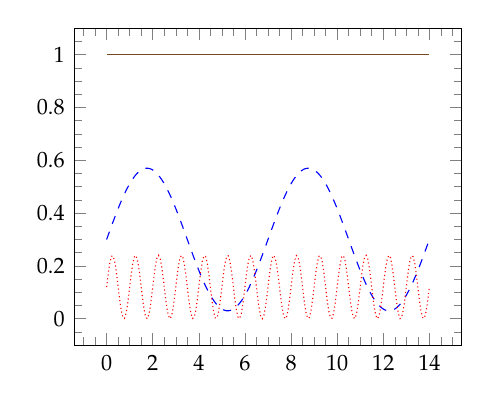
\begin{tikzpicture}
  \begin{axis}[
    domain=0:14, no markers, samples=200
    % xlabel = $x$, ylabel = $f(x)$
   ]
   \addplot+[dashed] {0.3 * (1 + 0.9 * sin(deg(2*pi*x/7)))}; \label{figref:w}
   \addplot+[densely dotted] {0.12*(1 + sin(deg(2*pi*x))}; \label{figref:s}
   \addplot+[solid] {1}; \label{figref:l}
  \end{axis}
 \end{tikzpicture}
 \caption{daily and multi-week variations of wind and solar power generation
	\(g^{N}_{w}(t)\)
	\autoref{figref:w} and \(g^{S}_{s}(t)\)
	\autoref{figref:s}, and a constant load (all in per-unit) \(L(t)\)
	\autoref{figref:l}.}
\label{fig:variations}
\end{wrapfigure}

Imagine a two-node Germany. The South can install solar panels with a capacity factor $c_s$ to cover its load $L^S$, while the North uses wind turbines that have a capacity factor $c_w$
to feed their load $L^N$. Figure \ref{fig:variations} shows approximations to the daily and multi-week variations of per-unit wind and solar power generation \(G^{N}_{w}(t)\) and \(G^{S}_{s}(t)\) and a constant load \(L^{N/S}(t)\):

\begin{align*}
 g_{w}^N(t) & = c_w(1+A_w \sin \omega_w t), \\
 g_{s}^S(t) & = c_s(1+A_s \sin \omega_s t), \\
L^{N/S}(t) & = A_{l}^{N/S}.
\end{align*}

The capacity factors and constants are
\begin{align*}
A_{l}^{N} & = 20 \si{\giga\watt}, & A_{l}^{S} & = 30 \si{\giga\watt},                                         \\
 c_w    & = 0.3,                & A_w     & = 0.9,                & \omega_w & = \frac{2\pi}{7 \text{d}}, \\
 c_s    & = 0.12,               & A_s     & = 1.0,                & \omega_s & = \frac{2\pi}{1 \text{d}}.
\end{align*}
\vspace{-0.3em}
For now, assume no power exchange between the regions and that the stores are lossless.

\begin{enumerate}[(a)]
 % (a)
 \begin{shaded}\item How much wind capacity $G^{N}_{w}$ must be installed in the North and solar capacity $G_s^S$ in the South so that on average generation matches demand?\end{shaded}

 In the North:

 $$\expect{L^N} = \expect{G^N_w \cdot g^N_w(t)}$$

 $$\Rightarrow \quad A^N_l = G^N_w\cdot c_w $$

 \DIVIDE{20}{0.3}\res

 $$\Rightarrow \quad G^N_w = \frac{A^N_l}{c_w} = \frac{20\si{\giga\watt}}{0.3} = \rd{\res}\si{\giga\watt}$$

 In the South:

 $$\expect{L^S} = \expect{G^S_s \cdot g^S_s(t)}$$

 $$\Rightarrow \quad A^S_l = G^S_s\cdot c_s $$

 \DIVIDE{30}{0.12}\res

 $$\Rightarrow \quad G^S_s = \frac{A^S_l}{c_s} = \frac{30\si{\giga\watt}}{0.12} = \rd{\res}\si{\giga\watt}$$

 % (b)
 \begin{shaded}\item For a system to work, generation must match demand not on average but at each location and each point in time. Storages are one way of ensuring this constraint with variable renewable generation. What is the amount of store and dispatch power capacity $G_{st,store}=\max(-\Delta(t))$ and $G_{st,dispatch} = \max \Delta(t)$ the storage units must have in the North and in the South to account for the mismatch $\Delta(t)=L(t)-G\cdot g(t)$?\end{shaded}

 In the North:

 \begin{align*}
  G_{s,storage,dispatch}^N & = \max ( \pm \Delta^N(t))                                                              \\
                           & = \max (\pm [L^N(t) - G^N_w \cdot g^N_w(t)])                                    \\
                           & = \max (\pm [L^N(t) - \frac{A^N_l}{c_w}\cdot c_w\cdot (1+A_w \sin \omega_w t)]) \\
                           & = \max (\pm [L^N(t) - A^N_l - A^N_l A_w \sin \omega_w t)])                      \\
                           & = \max (\pm [-A^N_l A_w \sin \omega_w t)])                                         \\
                           & = A^N_l A_w = 0.9 \cdot 20 \si{\giga\watt} = 18 \si{\giga\watt}
 \end{align*}

 In the South:

 \begin{align*}
  G_{s,storage,dispatch}^S & = \max ( \pm \Delta^S(t))                                                              \\
                           & = \max (\pm [L^S(t) - G^S_s \cdot g^S_s(t)])                             \\
                           & = \max (\pm [L^S(t) - \frac{A^S_l}{c_s}\cdot c_s\cdot (1+A_s \sin \omega_s t)]) \\
                           & = \max (\pm [L^S(t) - A^S_l + A^S_l A_s \sin \omega_s t)])                      \\
                           & = \max (\pm [A^S_l A_s \sin \omega_s t)])                                         \\
                           & = A^S_l A_s = 1.0 \cdot 30 \si{\giga\watt} = 30 \si{\giga\watt}
 \end{align*}

 % (c)
 \begin{shaded}\item What is the amount of energy capacity $E_{st}$ one needs for either storage in the North and in the South? The energy capacity is given by
 	
 	\begin{equation*}
 	E_{st} = \max_t e_{st}(t) = \max_t \int_{0}^{t} -\Delta(t') \;\mathrm{d}t'
 	\end{equation*}

 \end{shaded}

 In the North:

 \begin{align*}
  e_{st}^N(t) & = \int_{0}^{t} -\Delta^N(t') \;\mathrm{d}t' = \int_{0}^{t} A^N_l A_w \sin \omega_w t' \;\mathrm{d}t'           \\
           & = A^N_l A_w \frac{-\cos(\omega_w t')}{\omega_w}\Big|_0^t = A^N_l A_w \frac{1-\cos(\omega_w t')}{\omega_w}
 \end{align*}

 \begin{equation*}
  E_{st}^N = \max_t e_{st}(t) = \frac{2A^N_lA_w}{\omega_w} = \frac{2\cdot 20 \si{\giga\watt}\cdot 0.9}{2\pi} \cdot 7\cdot 24 \si{\hour} = 1 \si{\tera\watt\hour}
 \end{equation*}

 In the South:

 \begin{align*}
  e_{st}^S(t) & = \int_{0}^{t} -\Delta^S(t') \;\mathrm{d}t' = \int_{0}^{t} A^S_l A_s \sin \omega_s t' \;\mathrm{d}t'           \\
           & = A^S_l A_s \frac{-\cos(\omega_s t')}{\omega_s}\Big|_0^t = A^S_l A_s \frac{1-\cos(\omega_s t')}{\omega_s}
 \end{align*}

 \begin{equation*}
  E_{st}^S = \max_t e_{st}(t) = \frac{2A^S_lA_s}{\omega_s} = \frac{2\cdot 30 \si{\giga\watt}\cdot 1}{2\pi} \cdot 24 \si{\hour} = 230 \si{\giga\watt\hour}
 \end{equation*}

 % (d)
 \begin{shaded}\item Should they choose hydrogen or battery storages? And how much would it cost them? Is the South or the North paying more for their energy? Disregard losses!\end{shaded}

 \textbf{In the North:}

 The cost of renewable generation in the North is

 $$P_w^N=G^N_w \cdot 1200 \text{\EUR{}}\si{\per\kilo\watt}=80\cdot10^9\text{\EUR{}} $$

 The minimal (lossless) corresponding cost to supply constant demand by using hydrogen as storage technology are

 \begin{align*}
  P_h^N & = 750 \text{\EUR{}}\si{\per\kilo\watt} \cdot G_{storage,dispatch}^N + 10 \text{\EUR{}}/\text{kWh} \cdot E_{st}^N \\
        & = 13.5 \cdot 10^9 \eur + 10 \cdot 10^9 \eur                                                                                  \\
        & = 23.5 \cdot 10^9 \eur
 \end{align*}

 The minimal (lossless) corresponding cost to supply constant demand by using batteries as storage technology are:

 \begin{align*}
  P_b^N & = 300 \text{\EUR{}}\si{\per\kilo\watt} \cdot G_{storage,dispatch}^N + 200 \text{\EUR{}/kWh} \cdot E_{st}^N \\
        & = 5.4 \cdot 10^9 \eur + 200 \cdot 10^9 \eur                                                                                   \\
        & = 205.4 \cdot 10^9 \eur
 \end{align*}

 The minimal (lossless) total system cost using hydrogen storages accumulates to

 $$P_{w+h}^N = P_w^N + P_h^N = 104 \cdot 10^9\eur$$

 whereas the system cost using batteries are

 $$P_{w+b}^N = P_w^N + P_b^N = 285 \cdot 10^9\eur$$

 Thus, the North should choose hydrogen storages.\\~\\

 \textbf{In the South:}

 The cost of renewable generation in the South is

 $$P_s^S=G^S_s \cdot 600 \text{\EUR{}}\si{\per\kilo\watt}=150\cdot10^9\text{\EUR{}} $$

 The minimal (lossless) corresponding cost to supply constant demand by using hydrogen as storage technology are

 \begin{align*}
  P_h^S & = 750 \text{\EUR{}}\si{\per\kilo\watt} \cdot G_{storage,dispatch}^S + 10 \text{\EUR{}/kWh} \cdot E_{st}^S \\
        & = 22.5 \cdot 10^9 \eur + 2.3 \cdot 10^9 \eur                                                                                  \\
        & = 24.8 \cdot 10^9 \eur
 \end{align*}

 The minimal (lossless) corresponding cost to supply constant demand by using batteries as storage technology are:

 \begin{align*}
  P_b^S & = 300 \text{\EUR{}}\si{\per\kilo\watt} \cdot G_{storage,dispatch}^S + 200 \text{\EUR{}/kWh} \cdot E_{st}^S \\
        & = 9 \cdot 10^9 \eur + 46 \cdot 10^9 \eur                                                                                      \\
        & = 54 \cdot 10^9 \eur
 \end{align*}

 The minimal (lossless) total system cost using hydrogen storages accumulates to

 $$P_{s+h}^S = P_s^S + P_h^S = 175 \cdot 10^9\eur$$

 whereas the system cost using batteries are

 $$P_{s+b}^S = P_s^S + P_b^S = 204 \cdot 10^9\eur$$

 Thus, the South should also choose hydrogen storages.\\~\\

 \textbf{Cost comparison between North and South:}

 Without taking losses into account, both regions should choose hydrogen storages. Overall, the North can provide electricity at a lower rate than the South:

 $$P^N = \frac{104 \cdot 10^9 \eur}{20 \si{\giga\watt}} = 5 \cdot 10^9 \eur \si{\per\giga\watt}$$

 $$P^S = \frac{175 \cdot 10^9 \eur}{30 \si{\giga\watt}} = 6 \cdot 10^9 \eur \si{\per\giga\watt}$$

 Note that we can consider energy as $\si{\giga\watt}$ as we have a constant load! Otherwise, we would have to pay more attention!

 % (e)
\begin{shaded}\item Now we lift the restriction against transmission and allow the two regions to bridge their 500 km separation with a transmission line. Estimate the cost-optimal technology mix by assuming wind energy in the North is only stored in the North and solar energy in the South is likewise only stored in the South! What would happen if you dropped that assumption?\end{shaded}

Because $P_{w+h}^N < P_{w+h}^S$ there will be energy exports from North to South:

$$E^N > E^S \quad \text{and} \quad E^N + E^S = 50 \si{\giga\watt}$$

Note that we can consider energy as $\si{\giga\watt}$ as we have a constant load! Otherwise, we would have to pay more attention!

The total price of electricity is given by

\begin{align*}
P_{tot} & =\frac{ E^N \cdot P_{w+h}^N + E^S \cdot P_{s+h}^S + (E^N - E^S)\cdot 200 \eur\si{\per\kilo\watt}}{E^N + E^S}                                           \\
& = \frac{E^N \cdot P_{w+h}^N + (50\si{\giga\watt} - E^N) \cdot P_{s+h}^S + (2E^N - 50\si{\giga\watt})\cdot 200 \eur\si{\per\kilo\watt}}{E^N + E^S}      \\
& = \frac{E^N (P_{w+h}^N - P_{s+h}^S + 400 \eur \si{\per\kilo\watt}) + 50 \si{\giga\watt} (P_{s+h}^S - 200 \eur \si{\per\kilo\watt})}{E^N + E^S} \\
\end{align*}

Now, minimising the term for a choice of $E^N$ and filling in the costs calculated in the preceding tasks will yield

\begin{align*}
E^N & = 50 \si{\giga\watt}
\end{align*}

such that all power would be produced from wind in the North. This is because the term $(P_{w+h}^N - P_{s+h}^S + 400 \eur \si{\per\kilo\watt})$ is negative. The resulting total system cost is

\begin{align*}
\min P_{tot} & = \frac{-0.6 \cdot 50 \cdot 10^9 \eur + 5.8 \cdot 50 \cdot 10^9 \eur}{50 \si{\giga\watt}}  \\
& = \frac{260 \cdot 10^9 \eur}{50 \si{\giga\watt}} = 5.2 \cdot 10^9 \eur \si{\per\giga\watt}
\end{align*}

Compared to the weighted electricity cost of North and South without transmission

\begin{align*}
\min P_{tot} & = \frac{20\si{\giga\watt}\cdot 5 \cdot 10^9 \eur \si{\per\giga\watt} + 30\si{\giga\watt}\cdot 6 \cdot 10^9 \eur \si{\per\giga\watt}}{50 \si{\giga\watt}} \\
& = \frac{280 \cdot 10^9 \eur}{50 \si{\giga\watt}} = 5.6 \cdot 10^9 \eur \si{\per\giga\watt}
\end{align*}

the system cost could be reduced by approx.\ 7 \%.


 % (f)
  \begin{shaded}
 	\item What do you imagine would change if you considered the storage losses given in Table 1 in your results (a)-(d)?
 \end{shaded}
 
 To compensate for the energy losses wind and solar capacity $G_{w/s}$, store and dispatch power capacities $G_{storage,dispatch}$ and storage energy capacities $E_{st}$ have to increase. Since hydrogen storage has lower efficiencies than batteries, the optimal choice (particularly in the South) might change. You can prove that by taking into account the losses in your preceding calculations. The calculations including losses are uploaded in a seperate file.
 
 
\end{enumerate}

\end{document}
